\documentclass{article}
\usepackage[utf8]{inputenc}
\usepackage[serbian]{babel}

\usepackage{graphicx}
\graphicspath{ {./images/} }

\title{Klasifikacija muzičkih žanrova}
\author{Lucija Miličić \and Natalija Asanović}
\date{Avgust 2022.}

\begin{document}

\maketitle

\newpage

\section{Uvod}

Oznake muzičkih žanrova su korisne za organizovanje pesama, albuma i izvođača u šire grupe koje dele slične muzičke karakteristike. Kako količina muzike koja se izdaje na dnevnoj bazi sve više raste, raste i potreba za efikasnim određivanjem muzičkih žanrova. Cilj automatizacije muzičke klasifikacije je da izbor pesama bude brz i manje težak. Zbog toga klasifikacija muzičkih žanrova predstavlja jedan od važnih zadataka za mnoge aplikacije.

\subsection{Klasifikacija}
Zadatak klasifikacije jeste da odredi funkciju (klasifilacioni model) koja preslikava skup ulaznih atributa $X = (x^1, x^2, ..., x^k)$ u jednu od predefinisanih vrednosti $y$, gde je $y$ oznaka klase. 

Cilj formiranja modela je primena na materijal kod kojeg je vrednost atributa $y$ nepoznata, radi što preciznijeg predviđanja vrednosti $y$.

Ulazni podaci se obično dele u dva disjunktna skupa:
\begin{itemize}
    \item skup za trening - koristi se za formiranje modela
    \item skup za testiranje - koristi se za proveru ispravnosti modela
\end{itemize}

Moguće je uvesti i treći skup, skup za validaciju. On se koristi u toku formiranja modela, kako bi se izbegla preterana prilagođenost modela podacima.

\subsection{Tehnike klasifikacije}
Osnovne tehnike / metode klasifikacije su:
\begin{itemize}
    \item drveta odlučivanja
    \item neuronske mreze
    \item statistički zasnovane metode
    \item određivanje najbližeg suseda
    \item mašine sa potpornim vektorima
    \item ...
\end{itemize}

\subsection{Neuronske mreže}
Neuronske mreže trenutno predstavljaju metod mašinskog učenja sa najširim spektrom primena. Postoje različite vrste neuronskih mreža, koje su često specijalizovane za konkretne primene. 

Ono sto je zajedničko svim neuronskim mrežama jeste njihova struktura. Svaka neuronska mreža se sastoji od određenog broja elementarnih jedinica - neurona. Veštački neuron (eng. Artificial neuron - AN) predstavlja model biološkog neurona. Po analogiji sa biološkim neuronima, veštački neuroni jedni drugima prosleđuju
signale i izračunavaju nove signale na osnovu onih koji su im prosleđeni. Struktura povezanosti neurona
i način na koji oni vrše izračunavanja određuju o kakvoj mreži se
radi (npr. potpuno povezana neuronska mreza, konvolutivna neuronska mreza, rekurentna neuroska mreza, ...).

\subsubsection{Konvolutivne neuroske mreže}
Konvolutivne neuronske mreže imaju ulazni sloj, izlazni sloj, nekoliko skrivenih slojeva i veliki broj parametara, pomoću kojih mogu da nauče komplikovane obrasce.

Slojevi mogu biti \emph{konvolutivni} ili \emph{slojevi agregacije}. 

Neuronska mreža u svakom sloju uči određeni broj filtera. Skup filtera koji deluju nad istim ulazom nazivamo konvolutivnim slojem.

Slojevi agregacije služe za agregaciju informacija u cilju smanjenja količine izračunavanja i broja parametara u mreži.
\\

U nastavku rada pokazaćemo kako se klasifikuju muzički žanrovi korišćenjem konvolutivne neuronske mreže.

\section{Implementacjia}

\subsection{Ulazni podaci}
U implementaciji projekta je za obučavanje i testiranje modela korišćen skup podataka GTZAN koji sadrži 1000 pesama iz 10 muzičkih žanrova. Skup je podeljen u zasebne foldere po žanrovima: Blues, Classical, Country, Disco, Hip-hop, Jazz, Metal, Pop, Reggae, Rock, tako da se u svakom folderu nalazi po 100 pesama tog žanra, a svaka je dužine 30 sekundi. 

Pored samih audio fajlova, skup sadrži jos jedan folder organizovan na isti način sa vizuelnom reprezentacijom odgovarajućih pesama, kao i dva fajla u formatu .csv sa svojstvima istih pesama.

\subsubsection{Vizuelizacija audio fajlova}
Podaci kojima se pohranjuje konvolutivna neuronska mreža su slike kojima su predstavljene odgovarajuće pesme. Postoji više načina na koje se audio snimak može predstaviti u obliku slike, a najčešce korišćeni su:
\begin{itemize}
    \item grafik amplitude zvučnih talasa
    \item spektrogram
    \item spectral rolloff
    \item chroma feature
    \item zero crossing rate
\end{itemize}

U ovom projektu je za vizuelni prikaz zvuka korišćen spektrogram. Spektrogramom se predstavlja frekvencija signala, odnosno pomoću njega se moze pratiti ''glasnoća'' zvuka tokom vremena. Horizontalna osa spektrograma predstavlja vreme, vertikalna osa frekvenciju, dok treća dimenzija, odnosno boja na grafiku, predstavlja amplitudu.


Posmatranjem spektrograma iz različitih žanrova moguće je uočiti neke pravilnosti. Na sledećim primerima su izdvojene prve tri instance koje pripadaju redom žanrovima klasična muzika, rege i metal. Pored onoga što ljudsko oko može da uoči, neuronska mreža može da nauči i neke detalje koji nisu očigledni.

\begin{figure}[h]
\centering
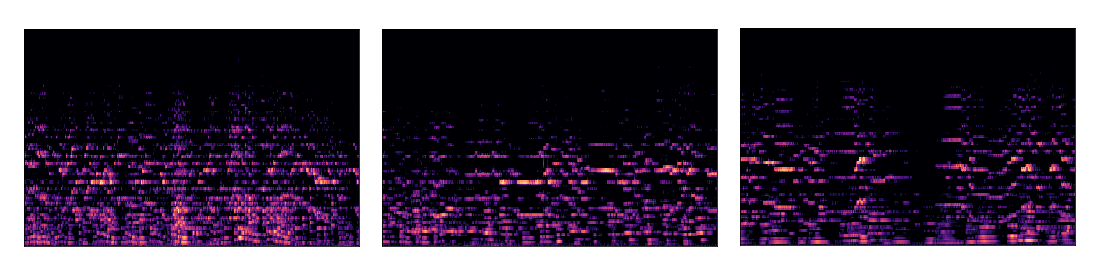
\includegraphics[scale=0.65]{classical}
\caption{Klasična muzika}
\end{figure}

\begin{figure}[h]
\centering
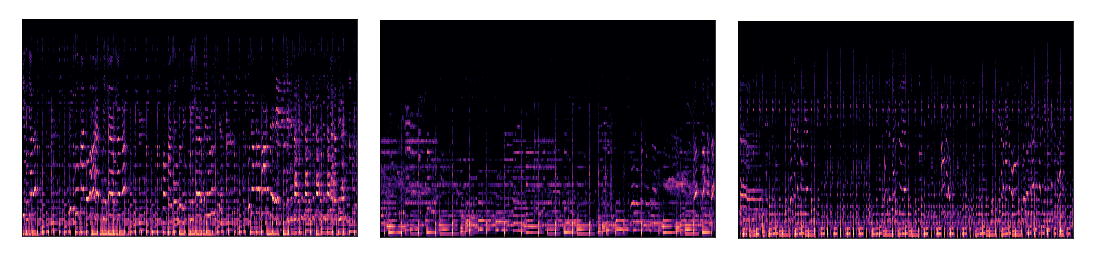
\includegraphics[scale=0.65]{reggae}
\caption{Rege}
\end{figure}

\begin{figure}[h]
\centering
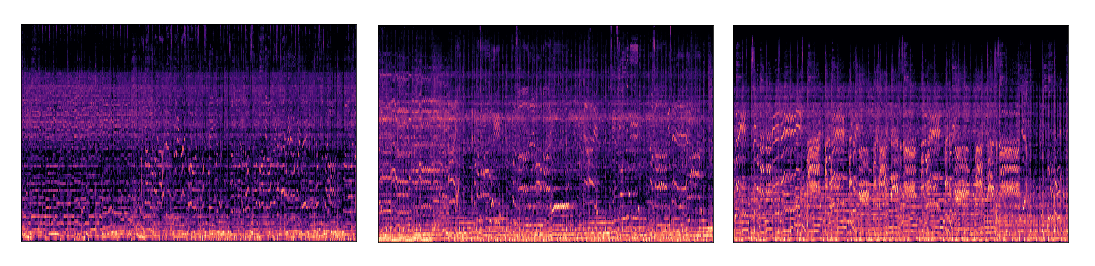
\includegraphics[scale=0.65]{metal}
\caption{Metal}
\end{figure}


\subsubsection{Akustičke karakteristike}

Osim vizuelne reprezentacije, audio snimke je moguce predstaviti i pomoću realnih brojeva. Fajlovi u formatu .csv sadrže razne odlike zvučnog signala u obliku tabele. Svakim redom u tabeli prikazane su odlike jedne pesme iz skupa. Atributi koji se mogu naći u njima su naziv i dužina pesme, ali i razlicite varijante MFCC, hromatske karakteristike (eng. chroma features), harmonija, tempo i sl. 

MFCC (eng. mel frequency cepstral coefficients) predstavlja mali skup karakteristika (obično oko 10 do 20) koje koncizno opisuju ukupan oblik spektralnog omotača, a najčešće se koriste za opisivanje boje zvuka.

Hromatske karakteristike takođe u kondenzovanom obliku predstavljaju tonski sadržaj audio signala, a veoma su značajne za prepoznavanje akorda i procenu harmonijske sličnosti.


\subsubsection{Priprema podataka}

Pre kreiranja modela neophodno je razumeti i pripremiti podatke koji se koriste. Skup podataka koji se korsiti u ovom projektu već sadrzi odgovarajuće fajlove sa akustičkim karakteristikama, kao i generisane spektrograme za svaku pesmu.

Spektrogrami su već pripremljeni, pa je potrebno samo učitati podatke i izvršiti podelu na trening i test skup. Za test skup izdvojeno je 30\% podataka i to ravnomerno iz svake klase.

Fajlove u formatu csv je potrebno dodatno pripremiti kako bi mogli da se koriste za treniranje modela. Za početak, neophodno je ukloniti naziv pesme iz skupa atributa, s obzirom na to da je njegova vrednost jednistvena za svaku instancu.

Sve ostale vrednosti su neki realni brojevi, međutim nemaju iste raspodele. Kako ne želimo da dajemo nekim atributima veći značaj u odnosu na druge, potrebno je izvršiti standardizaciju podataka, tj. svođenje vrednosti svih atributa na standardnu normalnu raspodelu.

Standardizaciju je moguće izvršiti korišćenjem funkcije StandardScaler iz biblioteke sklearn. Pošto test podaci treba da budu nepoznati, kako bismo ispravno mogli da ocenimo kvalitet dobijenog modela, onda njihove vrednosti ne smeju uticati na matematičko očekivanje i standardnu devijaciju koji se koriste za skaliranje. Zbog toga je neophodno prvo izvršiti podelu na trening i test skup, a zatim StandardScaler prilagoditi samo trening podacima. Isti parametri se zatim koriste za transformaciju oba skupa.

\subsection{Kreiranje neuronske mreže}

Centralni deo projekta predstavlja kreiranje i obučavanje neuronskih mreža. Na osnovu podataka treba izabrati koju mrežu je potrebno koristiti. Podatke koji predstavljaju spektrograme možemo posmatrati kao slike, odnosno matrice i koristiti ih za obučavanje konvolutivne mreže, dok podatke o akustičkim karakteristikama možemo videti kao vektore i stoga ih koristiti za treniranje potpuno povezane neuronske mreže.

\subsubsection{Parametri}

Potpuno povezana neuronska mreža se sastoji od 5 slojeva neurona, od kojih prva 4 koriste ''relu'' aktivacionu funkciju, dok poslednji koristi ''softmax''. Funkcija softmax slika ulazni vektor u vektor verovatnoća za svaku klasu. Dakle, za svaku instancu je na izlazu vektor iz kog mozemo pročitati za svaki muzicki žanr, koja je verovatnoća da ta instanca pripada baš tom žanru. Kao rezultat klasifikacije, biramo onaj žanr za koji je ta verovatnoća najveća.

Preprilagodjavanje je veoma česta pojava prilikom obučavanja neuronskih mreza. Ukazuje nam na to da se model ponaša veoma dobro na podacima koji su mu poznati, a znatno lošije na nepoznatim podacima. Za sprečavanje preprilagodjavanja korišćeni su takozvani dropout slojevi između svaka dva potpuno povezana sloja. Model je treniran na 200 epoha.

Struktura konvolutivne neuronske mreže se sastoji iz 3 konvolutivna sloja, a nakon svakog od njih se nalazi agregacioni sloj sa funkcijom maksimuma. Izlaz iz konvolutivnog dela mreže predstavlja ulaz u potpuno povezani deo koji se sastoji od dva sloja. Poslednji sloj takođe ima softmax aktivacionu funkciju.

Između ova dva dela se nalazi sloj za poravnavanje koji omogućava da se izlaz iz konvolutivnog dela, koji je dvodimenzioni, predstavi u obliku jednodimenzionog vektora. Takođe je korišćen jedan dropout sloj radi sprečavanja preprilagodjavanja i model je treniran na 20 epoha.

Za optimizator je u oba slučaja korišćen ''adam'', funkcija greške je kategorička unakrsna entropija i metrika za kvalitet modela je tačnost. 

\newpage

\section{Rezultati}

Procenu kvaliteta modela vršimo na osnovu test skupa. Ovaj skup sadrži instance koje su modelu nepoznate, tj. koje se nisu koristile za obučavanje. Zbog toga je ovakva ocena reprezentativna.

Dobijeni CNN model pokazuje tačnost oko 65\%, dok je tačnost potpuno povezane mreže oko 75\%. Pored tačnosti je za meru kvaliteta modela korišćena i matrica konfuzije.

\begin{figure}[h]
\centering
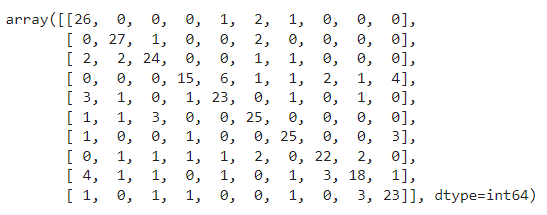
\includegraphics[scale=1.2]{matrix}
\caption{Matrica konfuzije CNN modela}
\end{figure}

Matrica konfuzije je takva da njen element $a_{ij}$ predstavlja broj instanci klase $i$ koje je dati model klasifikovao kao klasu $j$. Dakle, na dijagonali ove matrice se nalaze brojevi ispravno klasifikovanih instanci.

Detaljnijom analizom dobijene matrice konfuzije možemo da uočimo da model prilično dobro pravi razlike između razlicitih žanrova. Najčešće greške modela su pojedinačne pesme koje je klasifikovao kao instance nekog drugog žanra, odnosno, ne postoji učestalo mešanje bilo koje dve klase.

\section{Zaključak}

U ovom radu su predstavljena dva različita pristupa za rešavanje problema klasifikacije žanrova muzike. Prvi uključuje generisanje spektrograma na osnovu audio zapisa, koji se dalje tretira kao slika. Ovaj pristup koristi konvolutivnu neuronsku mrežu. Drugi pristup podrazumeva ekstrahovanje nekih značajnih akustičkih karakteristika, praćeno obučavanjem potpuno povezane neuronske mreže.

Važno je napomenuti da je korišćeni skup podataka relativno mali i da ne može u potpunosti da prikaže benefite ovih pristupa.

\end{document}
